
\documentclass[10pt]{article}

\def\Type{LessonDJ}
\def\TypeNum{Lesson 26}
\def\TypeTitle{Final Exam Review}
\def\Semester{Fall 2021} %Not Used 
\def\Course{MATH 1190 \& 1210}
\def\Targets{ }

\usepackage{preambleDJ}

%\usepackage{ragged2e}


%%%%%%%%%%%% BEGIN DOCUMENT %%%%%%%%%%%%%%%
%%%%%%%%%%%% BEGIN DOCUMENT %%%%%%%%%%%%%%%
%%%%%%%%%%%% BEGIN DOCUMENT %%%%%%%%%%%%%%%
%%%%%%%%%%%% BEGIN DOCUMENT %%%%%%%%%%%%%%%
%%%%%%%%%%%% BEGIN DOCUMENT %%%%%%%%%%%%%%%

%\usepackage{array}   % for \newcolumntype macro
%\newcolumntype{L}{>{$}l<{$}} % math-mode version of "l" column type
%\newcolumntype{C}{>{$}c<{$}} % math-mode version of "l" column type

%\newcommand{\rowstyle}[1]{\gdef\currentrowstyle{#1}}
%
%\usepackage{diagbox}

\def\sz{.2}

\begin{document}

\pagestyle{otherpages}
\thispagestyle{firstpage}
\vs{.25}
\section{Limits with Continuity and Forms}
\def\szz{1.15}
\enum{
\item \ltrm{\target{L2}}Evaluate the following limits using continuity or a specific form.  If you use continuity to evaluate a limit, to receive full credit, please provide sufficient explanation for why continuity can be used, including why the given function is continuous at the given point.
\enum{
\mpageTTh{.3}{.3}{.3}{
\item $\ds \limx \frac{x^3+e^x-2}{x^3+x^5}$
}{
Form:
}{
Value:
}
\vs{\szz}
\mpageTTh{.3}{.3}{.3}{
\item $\ds \lim_{x\to 0^-} \frac{x^3+e^x-2}{x^3+x^5}$
}{
Form:
}{
Value:
}
\vs{\szz}
\mpageTTh{.3}{.3}{.3}{
\item $\ds \lim_{x\to 2^+} \frac{x^3+e^x-2}{x^3+x^5}$
}{
Form:
}{
Value:
}
\vs{\szz}
\mpageTTh{.3}{.3}{.3}{
\item $\ds \limx \frac{\sqrt{9x^4+2x}-1}{2x^2+\sqrt{x}}$
}{
Form:
}{
Value:
}
\vs{\szz}
\mpageTTh{.3}{.3}{.3}{
\item $\ds \limx \frac{-\ln(x)+2}{2x^2+\sqrt{x}}$
}{
Form:
}{
Value:
}



}
}
\newpage
\section{Local and Absolute Extreme Values}
\enumR{
\item Consider the following function $f(x)$ and its derivative.\ltrm{\target{A2}}

\[f(x)=3x^5-5x^3\]%-(x-1)^4(15x^2+18x+7)\]

\[f'(x)=15x^2(x-1)(x+1)\]%10(1-x)^3(3x+1)^2\]

You are required to use methods we've learned in our course, such as the first derivative test, the second derivative test, the close interval method, or the first derivative test for absolute extrema, to solve this problem. In addition, you need to make sure the method you use is suitable for the question.
\begin{enumerate}
    \item Find all critical numbers of $f(x)$.

    \vfill

    \item For each critical number found in part (a), classify it as a local minimum, a local maximum, or neither. Fully justify your work.

    \vfill
    \vfill
    \vfill

    \item Find the $x$-values of all absolute extrema of $f(x)$ on the interval $[0, 2]$.

    \vfill
    \vfill
    \vfill
\end{enumerate}

}

\newpage
\section{Applications of the Derivative}
\enumR{
%\item \ltrm{\target{A2}}Let $f(x)=\ln|x^2-6x|$
%(Note: it is a logarithm of the \emph{absolute value} of $x^2-6x$).
%Additionally, note that $f'(x)=\dfrac{2x-6}{x^2-6x}$ and $f''(x)=\dfrac{-2x^2+12x-36}{(x^2-6x)^2}$.
%\begin{itemize}
%\item[(a)] Find all critical numbers of $f$.
%    
%    \vfill
%    \vfill
%    
%\item[(b)] For each critical number, determine whether a local maximum, a local minimum, or neither occurs at the critical number.
%
%    \vfill
%    \vfill
%    \vfill
%
%\item[(c)] Identify the absolute extrema of $f$ on the interval $[1,4]$.
%
%    \vfill
%    \vfill
%
%\end{itemize}
%
%\newpage

\item \ltrm{\target{A3}} A movie theater has found that if they price movie tickets at \$10 each, they can sell 100 tickets. If the price of each ticket is changed to $p$, then a total number of $n(p)=120-2p$ tickets are sold. There are only 120 seats in the theater.
 
What price should the movie theater sell the tickets at to maximize the revenue?

To receive full credit, make sure to clearly state the objective function, a domain/interval for optimization, and fully justify why price you've found maximizes the revenue. 

You are required to use a method we've learned in our course, such as the first derivative test, the second derivative test, the close interval method, or the first derivative test for absolute extrema, to solve this problem. In addition, you need to make sure the method you use is suitable for the question.
\newpage

\item \ltrm{\target{A3}}You are building five identical pens adjacent to each other with a
total area of $7500\ \text{m}^2$,
as shown in the following figure.
What dimensions should you use to minimize the amount of fencing?
\begin{center}
\begin{tikzpicture}[scale=1.2]
\draw (0,0) -- (5.0,0) -- (5.0,2.5) -- (0,2.5) -- (0,0);
\draw (1.0,0) -- (1.0,2.5);
\draw (2.0,0) -- (2.0,2.5);
\draw (3.0,0) -- (3.0,2.5);
\draw (4.0,0) -- (4.0,2.5);
\draw[dashed] (-.3,0) -- (-.3,2.5);
\draw (-.5,0) -- (-.1,0);
\draw (-.5,2.5) -- (-.1,2.5);
\node[font=\large] at (-.6,1.25) {$y$};
\draw[dashed] (0,2.8) -- (1,2.8);
\draw (0,2.6) -- (0,3);
\draw (1,2.6) -- (1,3);
\node[font=\large] at (.5,3.1) {$x$};
\end{tikzpicture}
\end{center}
}
\newpage

\section{Integrals}
\enumR{
\item \ltrm{\target{I1}} \enum{
 \item Let $r(t)$ represent the rate of energy produced by solar radiation per square meter, in kilowatts per square meter, or $kW/m^2$, on a given day, where $t$ is the number of hours since midnight.

    \begin{enumerate}
        \item[(i)] What is the unit of $\displaystyle\int_0^8 r(t)\, dt$?

        \vfill

        \item[(ii)] Explain the meaning of $\displaystyle\int_0^8 r(t)\, dt$ in this context.

        \vfill 
    \end{enumerate}

    \vfill

    \item When bleeding, a human heart still pumps blood, but the amount it pumps drops over time. In particular, the function $p(t)$ represents the amount of blood pumped by the heart per minute, where $t$ represents the number of minutes after the human starts bleeding.

    \begin{enumerate}
        \item[(i)] Based on this scenario, is $\displaystyle \int_0^5 p(t)\, dt$ positive, negative, or 0? No justification required.

        \vfill

        \item[(ii)] Write down an expression representing the amount of blood the heart pumps from 2 minutes after the start of bleeding to 10 minutes after the start of the bleeding.

        \vfill
    \end{enumerate}
    }


\newpage

\item \ltrm{\target{I2}}  Suppose the following values of definite integrals are given.

\[\int_{-1}^{2}g(x)\,dx=3\]

\[\int_{-3}^{-1}g(x)\,dx=1\]

\[\int_2^{-1}3(f(x)-g(x))\,dx=12\]

\[\int_{-3}^22(f(x)-g(x))\,dx=8\]

Find the value of the following definite integrals.

\tasksA{2}{
\task $\displaystyle\int_2^2 g(x)\, dx$

\task $\displaystyle\int_{-1}^2 f(x)\, dx$

\vspace{7cm}

\task $\displaystyle\int_{-3}^2 f(x)\, dx$
}
\newpage

\item \ltrm{\target{I3}}Assume $x>0$. Write down the indefinite integrals of the following expressions. 

Although no work is required, you are encouraged to include any work that shows your thought process. 

%constant, power, exponential, log, +C, algebraic manipulation

\begin{center}
         \begin{tabular}{l c r l c r}
            %
            $\displaystyle\int x^4+\log_2(10)\,dx$ & $=$ &\unlineb{1.5}{}{.35} &
            %
            %$\displaystyle\int \,dx$ & $=$ & \rule[-8pt]{1.5in}{0.4pt}\\[0.3in]
            %%%%%
            %$\displaystyle\int 15\,dx$ & $=$ & \rule[-8pt]{1.5in}{0.4pt} & 
            %%%%%
            $\displaystyle\int \dfrac{3}{x^8} \,dx$ & $=$ & \unlineb{1.5}{}{.35}  \\[1in]
            %%%%%
            $\displaystyle\int 3^x\,dx$ & $=$ & \unlineb{1.5}{}{.35}&
            %
            $\displaystyle\int \dfrac{1}{2x}\,dx$ & $=$ &  \unlineb{1.5}{}{.35} \\[1in]
            %%%%%
            $\displaystyle\int 4\sqrt{x}-e^x \,dx$ & $=$ &  \unlineb{1.5}{}{.35} & 
            %
            $\displaystyle\int \dfrac{1}{\sqrt[5]{x^3}} \,dx$ & $=$ &  \unlineb{1.5}{}{.35} \\[1in]
            %%%%%
        \end{tabular}\end{center}
        
\newpage

\item \ltrm{\target{I4}}For each of the following definite integrals, determine whether the Fundamental Theorem of Calculus can be applied to evaluate. 

If so, evaluate the integral using the FTC. There's no need to simplify your final answer.

If not, clearly indicate that and explain why.

\begin{enumerate}
    \item $\displaystyle\int_{-8}^{-1}\dfrac{1}{x}+e^x-\sqrt[3]{x}\, dx$

    \vfill

    \item $\displaystyle\int_{-8}^1\dfrac{1}{x}+e^x-\sqrt[3]{x}\, dx$

    \vfill
\end{enumerate}

}
\newpage

\section{Discrete and Continuous Probability Distributions} 
\itemI{
\item A {\em discrete probability distribution} is discrete because the set of outcomes is discrete: In the case of the sum of the roll of 2 dice die we had outcomes $\{2,3,4,\dots,12\}$.  In general, our set of outcomes will be  $\{x_1, x_2, x_3,\dots x_n\}$ where $n$ could also head towards infinity.
\item A {\em continuous probability distribution} is continuous because the set of outcomes of an experiment is continuous.  (e.g. measuring the height of a person, determining the wait time at the DMV, weighing a Roots Bowl, etc).
}
\enumR{
\item  \ltrm{\target{P1}}$X$ is the random variable that describes rolling two $6$-sided dice.The table below contains all possible rolls of two dice and the corresponding sums. You will find it helpful to answer the following questions.
\begin{center}
\renewcommand{\arraystretch}{1.4}
\begin{tabularx}{4.in}{|K{.4}{lightgray}|C{\sz}|C{\sz}|C{\sz}|C{\sz}|C{\sz}|C{\sz}|}\cline{1-7}
\rowcolor{lightgray}
 \diagbox{\hs{-.1}\text{\footnotesize  \bf Die 1}}{\hs{-.1}\text{\footnotesize \bf Die 2}}&1&2&3&4&5&6 \\ \cline{1-7}
 1&2&3&4&5&6&7 \\ \cline{1-7}
  2&3&4&5&6&7&8 \\ \cline{1-7}
3&4&5&6&7&8&9 \\ \cline{1-7}
4&5&6&7&8&9&10 \\ \cline{1-7}
5&6&7&8&9&10&11 \\ \cline{1-7}
6&7&8&9&10&11&12 \\ \cline{1-7}
\end{tabularx}
\end{center}
\tasksA{2}{
\task What is the support $S_X$? That is, what is the set of all possible outcomes from adding together the face values of two dice after one roll of the $2$ dice?  
\task How many different ways can two dice be rolled?   Note that  first rolling a $2$ and then a $1$ is distinct from first rolling a $1$ and then a $2$.   \vspace{1in}
\task* What is $p(4)=P(X=4)$?  It might be helpful to think about how many total combinations of dice rolls will yield a sum of $4$ relative to the total possible number of combinations that lead to our set of outcomes.\vs{1.25}\\
\task What is $P(X\leq 4)$?
\task What is $P(X\leq 4)+P(X\geq 5)$?
}
%%%%%%%%%
\newpage
%%%%%%%%%
\item  \ltrm{\target{P1}}$X$ is the random variable that describes rolling two $4$-sided dice.The table below contains all possible rolls of two dice and the {\em difference} between the second die and the first die.  You will find it helpful to answer the following questions.
\begin{center}
\renewcommand{\arraystretch}{1.4}
\begin{tabularx}{2.8in}{|K{.5}{lightgray}|C{\sz}|C{\sz}|C{\sz}|C{\sz}|} \cline{1-5}
\rowcolor{lightgray}
 \diagbox{\hs{-.1}\text{\footnotesize  \bf Die 1}}{\hs{-.1}\text{\footnotesize \bf Die 2}}&1&2&3&4 \\ \cline{1-5}
  1&0&1&2&3 \\ \cline{1-5}
    2&-1&0&1&2 \\ \cline{1-5}
3&-2&-1&0&1 \\ \cline{1-5}
4&-3&-2&-1&0 \\ \cline{1-5}
\end{tabularx}
\end{center}
\tasksA{2}{
\task What is the support $S_X$? That is, what is the set of all possible outcomes from subtracting together the face values of two dice after one roll of the $2$ dice?  
\task How many different ways can the two dice be rolled?   Note that  first rolling a $2$ and then a $1$ is distinct from first rolling a $1$ and then a $2$.   \vspace{1in}
\task What is $p(0)=P(X=0)$?  It might be helpful to think about how many total combinations of dice rolls will yield a difference of $0$ relative to the total possible number of combinations that lead to our set of outcomes.
\task Create a histogram containing probabilities for all elements of the support $S_{X}$. Note that you will want to label the horizontal axis with each element of the support.\\
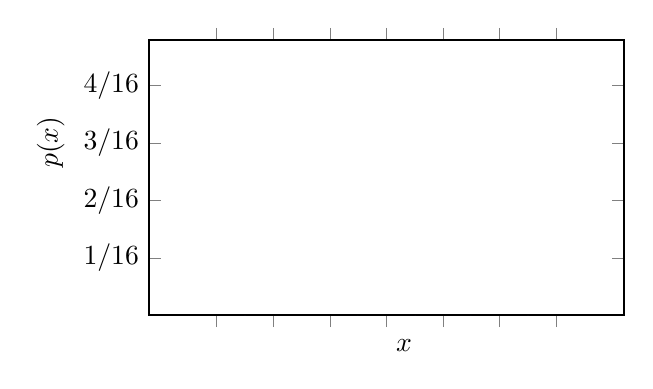
\begin{tikzpicture}
    \begin{axis}[
        ybar, % Specifies vertical bars
        bar shift=0,
        ymin=0, % Ensures bars start from zero
        xtick={1,2,3,4,5,6,7}, % Places x-axis ticks at data points
	xticklabels={,,,,,,}, % Custom x-axis labels
	%xticklabels={$-3$,$-2$,$-1$,$0$,$1$,$2$,$3$},
	ytick       = {1/16, 2/16, 3/16, 4/16},
            yticklabels =  {$1/16$,$2/16$,$3/16$, $4/16$},
        enlarge x limits={0.2}, % Adjusts spacing between bars and axis limits
            y label style={anchor=south west},
            ylabel={$p(x)$},
                        xlabel = {$x$},
		x label style={anchor=west},
		 ymin = 0, ymax = .3,
        bar width=20pt, % Adjusts the width of the bars
                    width = 3in, height=2in,
                    axis line style={thick, ->},
                    %enlarge x limits={1.2}
       % legend style={at={(0.5,-0.15)},anchor=north,legend columns=-1} % Legend positioning
    ]
 \addplot[fill=blue!40] coordinates {(1,0)  (2,0)  (3,0) (4,0) (5,0) (6,0) (7,0) };
 %\addplot[fill=blue!40] coordinates {(1,0.0625)  (2,0.125)  (3,0.1875) (4,0.25) (5,0.1875) (6,0.125) (7,0.0625) };
    \end{axis}
\end{tikzpicture}

\vs{.25}
\task Find the average difference for one roll of $2$ dice. That is, what's $E[X]$?
\task What is $Var(X)$? There's no need to simplify after setting this up.
}

}
%%%%%%%%%%%
\newpage
%%%%%%%%%%%


%%%%%%%%%%%%%%%%%%%  Bus stop problem  %%%%%%%%%%%%%%%
\enumR{
\item  \ltrm{\target{P2}}We're going to determine the probability of catching the bus at the stop on McIntyre between Monroe Hall and the amphitheater.  We assume that a bus comes every $10$ minutes and $T$ is a random variable that represents the wait time to catch the bus.  One probability density function (pdf) for this scenario is shown below. Note that   there's a low probability that a person will have to wait $0$ to $1$ minutes to catch the bus. There's also a low probability that a student will have to wait between $9$ and $10$ minutes to catch the bus.  But, there's a much higher probability that a person will catch the bus in between $4$ and $6$ minutes.  The pdf and graph of the pdf are below.\\
\mpageT{.5}{.5}{
\vs{.3}
\scalebox{1.2}{
$ \ds p(t)=\left\{
\begin{array}{ll}
\frac{1}{25}t&\qquad 0\leq t \leq 5\\
-\frac{1}{25}t+\frac{2}{5}&\qquad 5<t\leq 10
\end{array}
\right.
$
}
}{\centering
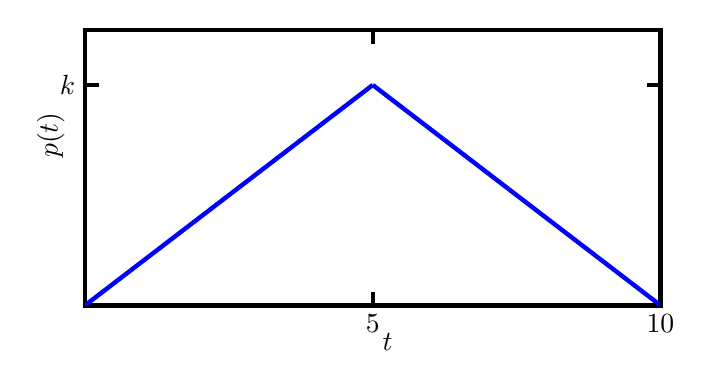
\begin{tikzpicture}
\begin{axis}[
	x label style={anchor=west},
xlabel={$t$},
xtick       = {5,10},
%xticklabels = {$10$,$20$,$30$},
xticklabel style={anchor=north},
y label style={anchor=west},
ylabel={$p(t)$},
%ytick=\empty,
%ytick       = {1/30},
ytick={0.2},
yticklabels = {$k$},
samples     = 320,
%domain      = -2.5:2.5,
%restrict y to domain=-6.5:6.5,
xmin =0, xmax = 10,
ymin = 0, ymax = .25,
axis line style = { ultra thick, -},
every major tick/.append style={ultra thick, black, major tick length=5pt},
width=3.5in, height=2in
%  grid=both, grid style=solid
]
    \addplot[domain=0:5, blue, ultra thick, mark=none]{1/25*x};
     \addplot[domain=5:10, blue, ultra thick, mark=none]{-1/25*x+2/5};
\end{axis}
\end{tikzpicture}
}
\tasksA{2}{
\task What's the probability that a person will wait $2.5$ minutes or less? That is, find $P(T\leq 2.5)$.
\task  What's the probability that a person will wait exactly $5$ minutes? That is, find $P(T= 5)$.
}
\vs{2}
\mpageT{.45}{.45}[\hs{.3}]{
\tasksAR{1}{
\task Let's now assume that it's equally likely that it will take $0-1$ minutes to catch the bus as $1-2$ minutes, as $2-3$ minutes, etc. That is, the wait time is uniformly distributed.  A probability density function that could represent this situation is below. Find a value of $k$ that will guarantee that this is a continuous probability distribution over $0\leq t\leq 10$.
}
}{\centering
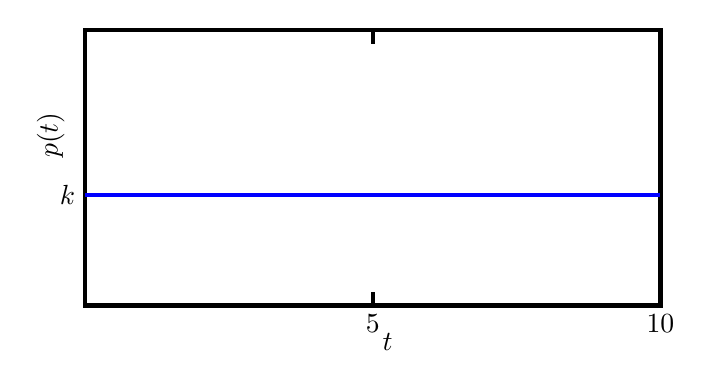
\begin{tikzpicture}
\begin{axis}[
	x label style={anchor=west},
xlabel={$t$},
xtick       = {5,10},
%xticklabels = {$10$,$20$,$30$},
xticklabel style={anchor=north},
y label style={anchor=west},
ylabel={$p(t)$},
%ytick=\empty,
%ytick       = {1/30},
ytick={0.1},
yticklabels = {$k$},
samples     = 320,
%domain      = -2.5:2.5,
%restrict y to domain=-6.5:6.5,
xmin =0, xmax = 10,
ymin = 0, ymax = .25,
axis line style = { ultra thick, -},
every major tick/.append style={ultra thick, black, major tick length=5pt},
width=3.5in, height=2in
%  grid=both, grid style=solid
]
    \addplot[domain=0:10, blue, ultra thick, mark=none]{0.1};
\end{axis}
\end{tikzpicture}
}

\newpage
\item \ltrm{\target{P2}}The expected value (or mean) of a continuous random variable $X$ is $\ds \mu=E[X]=\int_1^5k\;dx$ where $k$ is an unknown constant that we will find later. 
\tasksA{2}{
    \task  What is the probability density function $p(x)$? Your answer will involve $k$.
    \task Find the value of $k$ to ensure that $p(x)$ is a pdf.  {em Hint}:  You will want to use the fact that $\ln(1)=0$
    \vs{2}
    \task Find the cumulative distribution function (CDF) $F(x)$.
    \task Use $F(x)$ to find $P(X \leq 4)$.
    \vs{2}
    \task Find $\ds \mu=E[X]$ 
    \task Find $Var(X)$
    }



%\newpage
%%%%%%%%%%%%%%%%%%%  Extra Problem  %%%%%%%%%%%%%%%
%\item Gaming problem \#$1$  
%\itemI{
%\item {\bf Experiment} Bet $\$40$ each time coin is flipped. Heads means bettor receives original bet back and an additional $\$40$. Tails means bettor loses original bet.
%\item {\bf Discrete Random Variable}  $X$ is the random variable describing how much money you have after (randomly) flipping a coin only once. 
%\item Start with $\$40$
%}
%\tasksA{2}{
%	\task What is sample space of Experiment 1 of  flipping coin only once?
%	\task What is the support $S_X$?\vs{1}
%
%	\task* Create a histogram that represents the probability of arriving at each of the outcomes in $S_X$. 
%	\graphicsL{axesHistogram}{2.}	
%	}
%	\vs{.5}
%\item Gaming problem \#$2$  
%\itemI{
%\item {\bf Experiment} Bet $\$40$ each time coin is flipped. Heads means bettor receives original bet back and an additional $\$40$. Tails means bettor loses original bet.
%\item {\bf Discrete Random Variable}  $X$ is the random variable describing how much money you have after (randomly) flipping a coin twice. 
%\item Start with $\$80$
%}
%\tasksA{2}{
%	\task What is sample space of Experiment 2 of  flipping coin twice?
%	\task What is the support $S_X$?\vs{1}
%
%	\task* Create a histogram that represents the probability of arriving at each of the outcomes in $S_X$. 
%	\graphicsL{axesHistogram}{2.}	
%	}
%	\newpage
%	\item {\bf Challenge Question} (only if time): Start with \$120 and bet  $\$40$ each time coin is flipped. Heads means bettor receives original bet back and an additional $\$40$.  Player stops either when they run out of money or when they reach $\$200$. Which is more likely-- they run out of funds first or reach $\$200$ first?  An informal argument using  probabilities is ok here.  For a bigger challenge, find the probability that they run out of funds first. \vs{4}
	
}

\end{document}